\subsubsection{Fundamento}

El detector de marcadores implementa un algoritmo basado en segmentación por umbralización y análisis morfológico de contornos. Este enfoque clásico de visión por computadora explota el alto contraste entre elementos oscuros (cintas negras) y fondo claro mediante procesamiento en el espacio de color HSV, sin requerir aprendizaje automático supervisado.

El sistema mecánico del robot presenta holguras acumulativas que generan errores de posicionamiento de hasta ±5 milímetros respecto a la posición comandada. Estos errores resultan incompatibles con los requerimientos de precisión para las operaciones de cosecha, que exigen tolerancias inferiores a ±1 milímetros. Para compensar estas desviaciones se implementó un sistema de corrección visual basado en la detección de marcadores de referencia.

Los marcadores consisten en cintas adhesivas negras de 18 milímetros de ancho adheridas sobre la superficie de los tubos de PVC blanco. Esta configuración proporciona un contraste entre el elemento oscuro y el fondo claro, facilitando su detección mediante técnicas de procesamiento de imágenes. La selección de cintas adhesivas como elemento de marcado se fundamentó en su bajo costo de implementación, su robustez ante las condiciones, y la facilidad de instalación sin modificaciones estructurales del sistema.

Las cintas se disponen de forma vertical como se puede observar en la Figura \ref{fig:configuracion_cintas}, alineadas con los espacios de cultivo. Esta disposición permite al robot identificar su posición relativa tanto en el eje \textbf{X} (posición media de la cinta) como en el eje \textbf{Y} (arista base de la cinta) mediante la detección de los marcadores.

\begin{figure}[H]
\centering
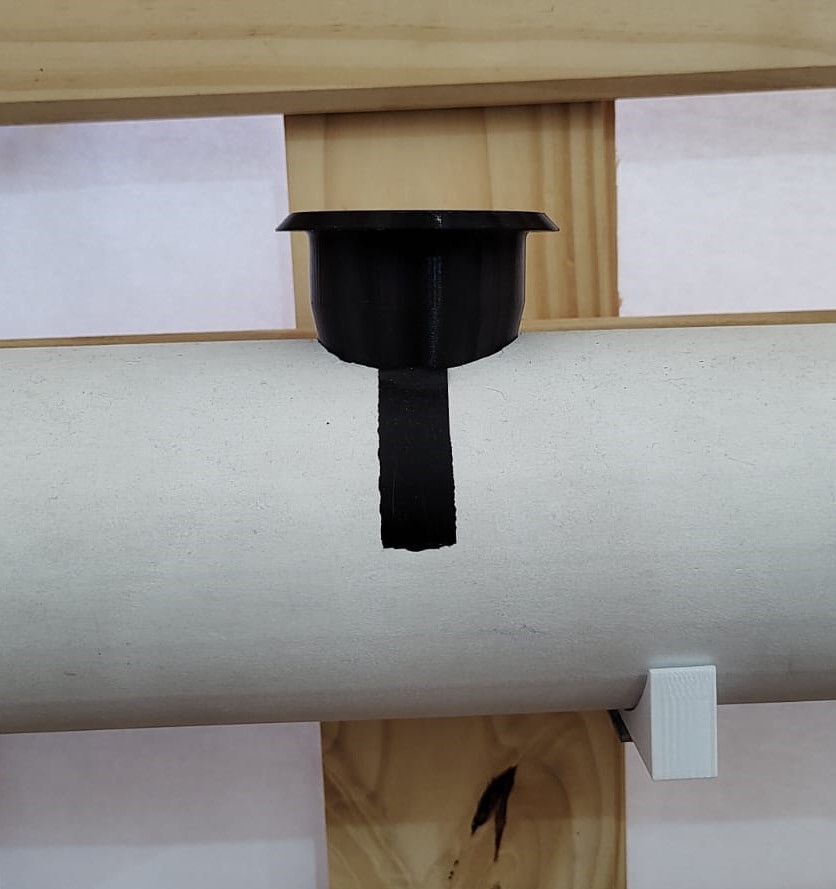
\includegraphics[width=0.50\textwidth]{imagenes/configuracion_cintas_referencia.jpg}
\caption{\textit{Disposición de cintas de referencia horizontal y vertical en el sistema hidropónico}}
\label{fig:configuracion_cintas}
\end{figure}
